\documentclass[aps,showpacs,superscriptaddress]{revtex4}
\usepackage[pdftex]{graphicx}   % for figures
\usepackage{epstopdf}
\usepackage{dcolumn}
\usepackage{bm}	
\usepackage{textcomp }
\usepackage{amsmath}			% Mode mathematique
\usepackage{amsfonts}			% Polices mathematiques
\usepackage{amssymb}
\usepackage{gensymb}		% Symboles mathematiques
\usepackage{latexsym}		% Symboles mathematiques avances
\usepackage{color}
% Asked by the editor
%%%%%%%%%%%%%%%%%%%%%
\usepackage[nomarkers,figuresonly]{endfloat}
\linespread{2}
%%%%%%%%%%%%%%%%%%%%%
\begin{document}

\title{\textcolor{blue}{Growth of concomitant laser-driven} collisionless and resistive electron filamentation instabilities over large spatiotemporal scales
}


\author{C. Ruyer}\email{charles.ruyer@cea.fr}
\affiliation{LULI - CNRS, CEA, UPMC Univ Paris 06: Sorbonne Universit\'e, Ecole Polytechnique, Institut Polytechnique de Paris - F-91128 Palaiseau Cedex, France}
\affiliation{SLAC National Accelerator Laboratory, Sand Hill Road, Menlo Park, California, USA}
\affiliation{CEA, DAM, DIF, F-91297 Arpajon, France}
\author{S. Bolanos }
\affiliation{LULI - CNRS, CEA, UPMC Univ Paris 06: Sorbonne Universit\'e, Ecole Polytechnique, Institut Polytechnique de Paris - F-91128 Palaiseau Cedex, France}
\author{B. Albertazzi}
\affiliation{LULI - CNRS, CEA, UPMC Univ Paris 06: Sorbonne Universit\'e, Ecole Polytechnique, Institut Polytechnique de Paris - F-91128 Palaiseau Cedex, France}
\affiliation{INRS-EMT, Varennes, Qu\'ebec, Canada}
\author{S.~N. Chen}
\affiliation{ELI-NP, ”Horia Hulubei” National Institute of Physics and Nuclear Engineering, Bucharest - Magurele, Romania }
\affiliation{Institute of Applied Physics, 46 Ulyanov Street, 603950 Nizhny Novgorod, Russia}
\author{P. Antici}
\affiliation{INRS-EMT, Varennes, Qu\'ebec, Canada}
\author{J. B\"oker}
\affiliation{Institut f\"ur Laser-und Plasmaphysik, Heinrich-Heine-Universit\"at, D\"usseldorf, Germany}
\author{V. Dervieux}
\affiliation{LULI - CNRS, CEA, UPMC Univ Paris 06: Sorbonne Universit\'e, Ecole Polytechnique, Institut Polytechnique de Paris - F-91128 Palaiseau Cedex, France}
\affiliation{CEA, DAM, DIF, F-91297 Arpajon, France}
\author{ L. Lancia}
\affiliation{LULI - CNRS, CEA, UPMC Univ Paris 06: Sorbonne Universit\'e, Ecole Polytechnique, Institut Polytechnique de Paris - F-91128 Palaiseau Cedex, France}
\affiliation{Dept. SBAI, Universita di Roma ``La Sapienza'', Via A. Scarpa 14 00181 Rome, Italy}
\author{M. Nakatsutsumi}
\affiliation{LULI - CNRS, CEA, UPMC Univ Paris 06: Sorbonne Universit\'e, Ecole Polytechnique, Institut Polytechnique de Paris - F-91128 Palaiseau Cedex, France}
\address{European XFEL GmbH, Holzkoppel 4, Schenefeld D-22869, Germany}
\author{L. Romagnani}
\affiliation{LULI - CNRS, CEA, UPMC Univ Paris 06: Sorbonne Universit\'e, Ecole Polytechnique, Institut Polytechnique de Paris - F-91128 Palaiseau Cedex, France}
\author{R. Shepherd}
\affiliation{Lawrence Livermore National Laboratory, Livermore, CA 94550, USA}
\author{M. Swantusch}
\affiliation{Institut f\"ur Laser-und Plasmaphysik, Heinrich-Heine-Universit\"at, D\"usseldorf, Germany}
\author{M. Borghesi}
\affiliation{School of Mathematics and Physics, Queen's University Belfast, United Kingdom}
\author{O. Willi}
\affiliation{Institut f\"ur Laser-und Plasmaphysik, Heinrich-Heine-Universit\"at, D\"usseldorf, Germany}
\author{H. P\'epin}
\affiliation{INRS-EMT, Varennes, Qu\'ebec, Canada}
\author{M. Starodubtsev}
\affiliation{Institute of Applied Physics, 46 Ulyanov Street, 603950 Nizhny Novgorod, Russia}
\author{M. Grech}
\affiliation{LULI - CNRS, CEA, UPMC Univ Paris 06: Sorbonne Universit\'e, Ecole Polytechnique, Institut Polytechnique de Paris - F-91128 Palaiseau Cedex, France}
\author{C. Riconda}
\affiliation{LULI - CNRS, CEA, UPMC Univ Paris 06: Sorbonne Universit\'e, Ecole Polytechnique, Institut Polytechnique de Paris - F-91128 Palaiseau Cedex, France}
\author{L. Gremillet}\email{laurent.gremillet@cea.fr}
\affiliation{CEA, DAM, DIF, F-91297 Arpajon, France}
\author{J. Fuchs}\email{julien.fuchs@polytechnique.edu}
\affiliation{LULI - CNRS, CEA, UPMC Univ Paris 06: Sorbonne Universit\'e, Ecole Polytechnique, Institut Polytechnique de Paris - F-91128 Palaiseau Cedex, France}
\affiliation{Institute of Applied Physics, 46 Ulyanov Street, 603950 Nizhny Novgorod, Russia}


\begin{abstract}
\textcolor{blue}{Collective processes in plasmas often induce micro-instabilities that play an important role in many space or laboratory plasma environments. Particularly notable is the Weibel-type current filamentation instability, which is believed to drive the creation of collisionless shocks in weakly magnetized astrophysical plasmas. Here, this instability class is studied through interactions of ultraintense and short laser pulses with solid foils, leading to localized generation of MeV electrons. Proton radiographic measurements of both low- and high-resistivity targets show two distinct, superimposed electromagnetic field patterns arising from the interpenetration of the MeV electrons and the background plasma. Particle-in-cell simulations and theoretical estimates suggest that the collisionless Weibel instability building up in the dilute expanding plasmas formed at the target surfaces causes the observed azimuthally symmetric electromagnetic filaments. For a sufficiently high resistivity of the target foil, an additional resistive instability is triggered in the bulk target, giving rise to radially elongated filaments. The data reveal the growth of both filamentation instabilities over large temporal (tens of picoseconds) and spatial (hundreds of microns) scales.}
\end{abstract}
\maketitle

The interaction of high-energy, charged particle flows with plasmas is a fundamental question in plasma physics and, more generally, physical kinetics. The energy and momentum transfers between the plasma species are mediated by either Coulomb collisions~\cite{Shkarofsky_1966} or collective processes~\cite{Belmont_2013}, depending on the density and velocity distributions of the plasma populations. Collective processes often give rise to plasma micro-instabilities, i.e., growing electrostatic or electromagnetic fluctuations that develop at kinetic electron or ion scales in systems with multi-stream or anisotropic momentum distributions~\cite{Davidson_1983}. 

An important class of instabilities is the Weibel-type current filamentation instability, which originates from thermal anisotropies~\cite{PRL_Weibel_1959} or relative drifts between the plasma species~\cite{POF_Fried_1959}. It generates kinetic-scale electromagnetic fields, which tend to deflect and thermalize the interacting particles \cite{POF_Davidson_1972, PRL_Lee_1973, PRL_Adam_2006}. This mechanism is drawing strong interest in high-energy astrophysics as it is suspected to underlie the formation of collisionless shocks, and their related phenomena, in weakly magnetized (electron-ion or electron-positron) plasmas~\cite{RPP_Marcowith_2016}. It is also a possible mediating agent for magnetizing the intergalactic medium \cite{APJ_Schlickeiser_2003}.

Much effort is currently expended in designing experiments to investigate this instability in the laboratory, either using conventional accelerator beams \cite{PRL_Allen_2012}, or laser-generated beams \cite{PRL_Fox_2013, NP_Huntington_2015}, the latter being favored by many teams for the high-density, high-current beams that can be obtained, as well as for the variety of plasma conditions that can be simultaneously produced using auxiliary beams. 

In the case addressed here, where ultraintense ($>10^{18}\,\rm W.cm^{-2}$) short ($\lesssim 1\,\rm ps$) laser pulses impinging onto overcritical targets are used to generate mega-ampere currents of energetic (MeV) electrons, the Weibel/current filamentation instability spontaneously arises from the interpenetration of these fast electrons and the background plasma. Around the laser spot, the plasma is heated to very high (keV) temperatures, and hence the instability is mainly collisionless and builds up at electron kinetic scales \cite{PRL_Adam_2006}. Note that in this region the Biermann battery mechanism will drive a large-scale magnetic field \cite{RSI_Albertazzi_2015}, adding up to that produced by the Weibel instability \cite{PRL_Schoeffler_2014}.
As of now, experimental evidence for the resulting small-scale surface magnetic fields has been obtained through high-resolution polarigrams \cite{PNAS_Mondal_2012} or proton radiographs \cite{PRL_Romagnani_2019} in the vicinity of the irradiated region. The fast electrons, however, can also be prone to further filamentation when propagating through the target bulk. The resistive character of the cold plasma electrons making up the fast-electron-neutralizing return current \cite{POP_Gremillet_2002} then leads to larger magnetic filaments \cite{JPP_Fiore_2010} and enhanced fast-electron scattering \cite{POP_Yang_2016}. Such resistive filamentation has been diagnosed either indirectly, from spatial modulations of the sheath-field-accelerated protons \cite{PRL_Fuchs_2003, PRL_MacLellan_2013}, or directly, from the optical emission induced by the fast electrons  \cite{PRL_Storm_2009}. Finally, the collisionless Weibel instability can also arise from fast electrons interacting with micron-scale-length plasma gradients at the target surfaces~\cite{PRE_Wei_2004, PRL_Quinn_2012, NJP_Metzkes_2014, PRL_Gode_2017, NJP_Scott_2017}.

\begin{figure}[tbh!]
%\centerline{
%\begin{tabular}{c}
%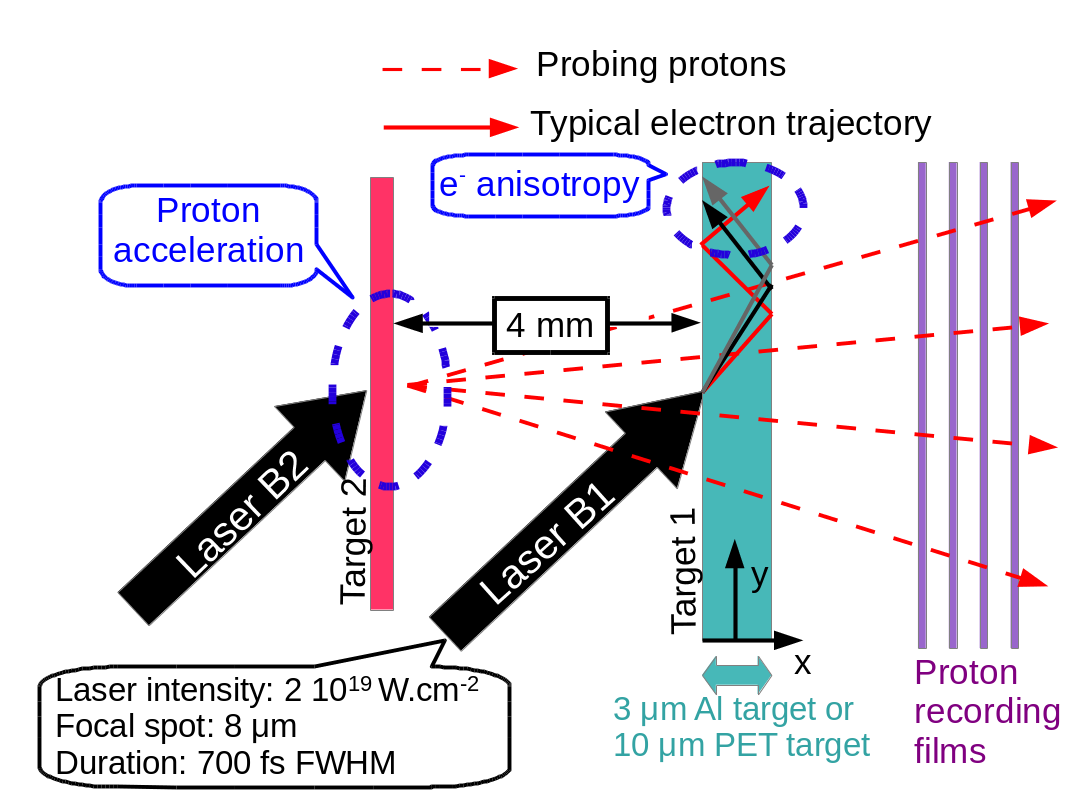
\includegraphics[scale=0.25]{sketch.png}
%\end{tabular}}
\caption{\label{fig:xp} \textbf{Sketch of the experimental setup.} 
\textcolor{blue}{The fast electrons (plain arrows) generated by irradiation of target 1 (in green) by laser B1 trigger electromagnetic fluctuations as they circulate through the target (composed of Al or of Polyethylene terephthalate (PET), a plastic polymer composed of (C10H8O4) monomers). These fluctuations deflect the probe protons (red dashed arrows) accelerated from target 2 (in red) by laser B2, and sent through target 1. The modulated transverse profiles of the probe protons are imaged as a function of their energy by a stack of recording films (in purple).}}
\end{figure}

The experimental and numerical data gathered so far seem to suggest that magnetic filaments only form relatively near the laser axis (over a few tens of microns), where the fast electron density, and therefore the overall plasma anisotropy, are initially at their highest. Furthermore, in contrast with simulation results \cite{POP_Heron_2015, POP_Yang_2016}, there has been as yet no observation of the simultaneous development of the collisionless and resistive variants of the instability in, respectively, the surface and inner regions of dense targets. Here, unlike previous studies, we present measurements and numerical simulations demonstrating: (i) filamentary magnetic-field generation by fast electrons over much larger scales than previously thought possible, both in space (hundreds of microns, i.e., far away from the laser focal spot vicinity and far from the region where the Biermann magnetic field develops) and time (tens of ps), and (ii) the simultaneous development of the collisionless and resistive types of filamentation in different areas of the target. \textcolor{blue}{These data, together with analytical modelling, allow us to untangle the conditions for their occurrence and differential development, depending on the target material traversed by the fast electrons.}

Our measurements make use of the proton radiography technique (see Fig.~\ref{fig:xp} and Methods), by means of two high-temporal-contrast, short-pulse laser beams, B1 and B2. More details on the setup can be found in Ref.~\cite{RSI_Albertazzi_2015}.
\textcolor{blue}{B1} irradiates \textcolor{blue}{target 1} (a $3\,\rm \mu m$ thick Al or a $10\,\rm \mu m$ thick PET foil) at an angle of $31^\circ$ to the target normal (in the horizontal plane), while \textcolor{blue}{B2} generates the \textcolor{blue}{probe} protons from target \textcolor{blue}{2}. Depending on \textcolor{blue}{target 1}'s material (Al being a conductor, PET being an insulator), two types of electromagnetic field patterns are observed to arise, which kinetic simulations indicate are induced by collisionless and resistive current filamentation instabilities. These are triggered as the fast electrons, respectively, recirculate in the low-density \textcolor{blue}{plasmas} expanding into the vacuum and drift away from the laser spot into the cold, solid-density target bulk. As will be detailed in Figs.~\ref{fig:pic} and \ref{fig:kxy}, such instabilities generate electromagnetic structures consistent with the experimental observations in the Al and PET foils in terms of field strength \textcolor{blue}{($\sim 5\,\rm T$)}, wavelength ($\sim 100\,\rm \mu m$), as well as spatiotemporal evolution (instability triggered a few $100\,\rm \mu m$ away from the focal spot, $\sim 1\,\rm ps$ after the main laser drive).
%
\begin{figure*}[tbh!]
%\begin{tabular}{cc}
%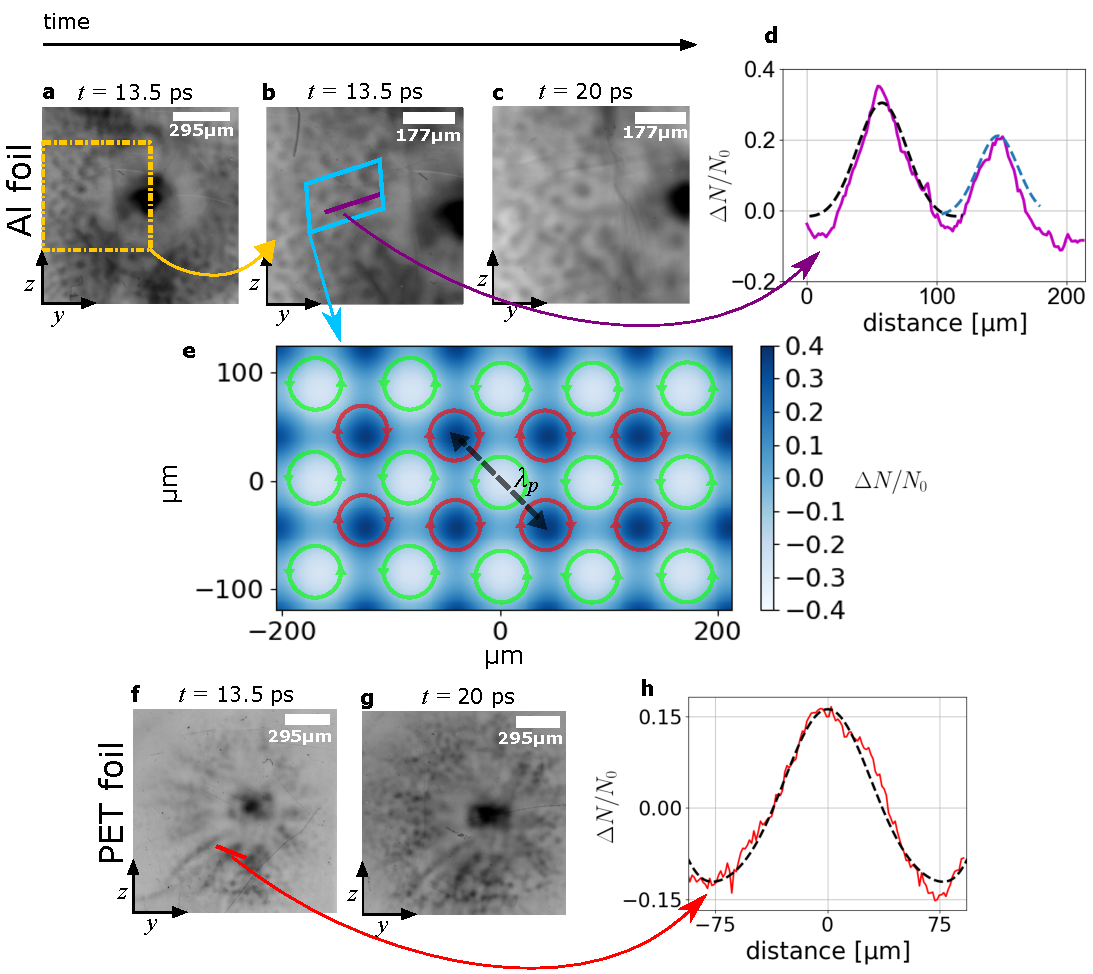
\includegraphics[width=0.7\textwidth]{panel_v10.png}
%\end{tabular}
 \caption{\textcolor{blue}{
\textbf{Proton radiographs showing filamentation instabilities.
}
{\bf a}-{\bf c}, Radiographs at various times, obtained with an Al foil as target 1. The time origin $t=0$ is when laser B1 irradiates target 1.} Darker and lighter areas correspond to increased and depleted proton dose, respectively \cite{RSI_Albertazzi_2015}. 
{\bf b},{\bf c}, Closeups of the off-center region delimited by the yellow dashed square in {\bf a}. Small-scale modulations are observed to develop after $\sim 1\,\rm ps$.
{\bf d}, Normalized proton dose profile along the purple line in {\bf b} (purple solid curve) and \textcolor{blue}{fitted} synthetic dose profiles (black and blue dashed curves) (see Methods).
{\bf e}, Schematic pattern of the magnetic field lines (circular arrows) \textcolor{blue}{expected to} develop in the zone delimited by the blue box in {\bf b}, overlaid on the resulting (simulated) proton dose modulation $\Delta N/N_0$ (pseudocolor map) obtained without taking account of the radial electric field. Red and green loops indicate magnetic field lines of opposite polarity.
{\bf f},{\bf g}, Proton radiographs obtained with a PET foil as \textcolor{blue}{target 1}. On top of a small-scale dotted pattern akin to that seen in {\bf a}-{\bf c}, one observes radial streaks extending from the central laser spot. 
{\bf h}, Normalized proton dose profile along the red line in {\bf f} (red solid curve) and synthetic  fitted dose profile (black dashed curve) (see Methods).
All spatial scales refer to the \textcolor{blue}{target 1} plane.
}
\label{fig:radio}
\end{figure*}

On the radiographs shown in Fig.~\ref{fig:radio}, the dark and white regions result from, respectively, accumulation and depletion of the \textcolor{blue}{probe} protons through the quasistatic fields induced around \textcolor{blue}{target 1}. All frames associated with either the Al (Figs.~\ref{fig:radio}a-c) or PET (Figs.~\ref{fig:radio}f-g) foil, corresponding to different energies of the \textcolor{blue}{probe} protons, and hence to different times-of-flight between \textcolor{blue}{target 2 and target 1} (as indicated above each frame), are taken from a single shot. The irradiated region can be located by the large black area encircled by a white ring of $\sim 300\,\rm \mu m$ radius, delineating the large-scale $B$-field created by the Biermann battery on the surfaces of \textcolor{blue}{target 1} (see Ref.~\cite{RSI_Albertazzi_2015} and references therein). Remarkably, the radiographs also evidence a small-scale spotted pattern, developing from $\sim 400\,\rm\mu m$ to $\gtrsim 700\,\rm \mu m$ away from the focal spot, with a typical wavelength  $\lambda_p \simeq 100\,\rm \mu m$ (see lineout in Fig.~\ref{fig:radio}d) and lasting at least $43\,\rm ps$ (see Supplementary Figure 2b). These structures, absent without \textcolor{blue}{B1 irradiating target 1} (the protons then exhibit a homogeneous dose, see Fig.~2i of Ref.~\cite{RSI_Albertazzi_2015}), are observed within the first ps following the laser peak (see  Supplementary Figure 2a). Moreover, they \textcolor{blue}{first arise to the left}  
of the irradiated region, i.e., in a domain towards which the hot electrons are expected to be preferentially flowing. Figure~\ref{fig:radio}e displays an idealized pattern of (azimuthal) magnetic and (radial \textcolor{blue}{and weaker}) electric fields (see Methods), yielding a synthetic radiograph (pseudocolor map) qualitatively matching the experimental data. Note that the magnetic structures inferred in Ref.~\cite{PRL_Gode_2017} from modulations in the accelerated proton beam are consistent with \textcolor{blue}{our measurements},
but with a much smaller wavelength and larger amplitude due to their proximity to the laser spot.

The radiographs of the PET targets reveal a dotted pattern qualitatively similar to that seen in Al. Yet they also feature larger-scale radial dark streaks, which suggests that another mechanism for electromagnetic field generation, absent or weakly operative in Al, is here diagnosed on the line of sight of the \textcolor{blue}{probe} protons.

\begin{figure*}[tbh!]
%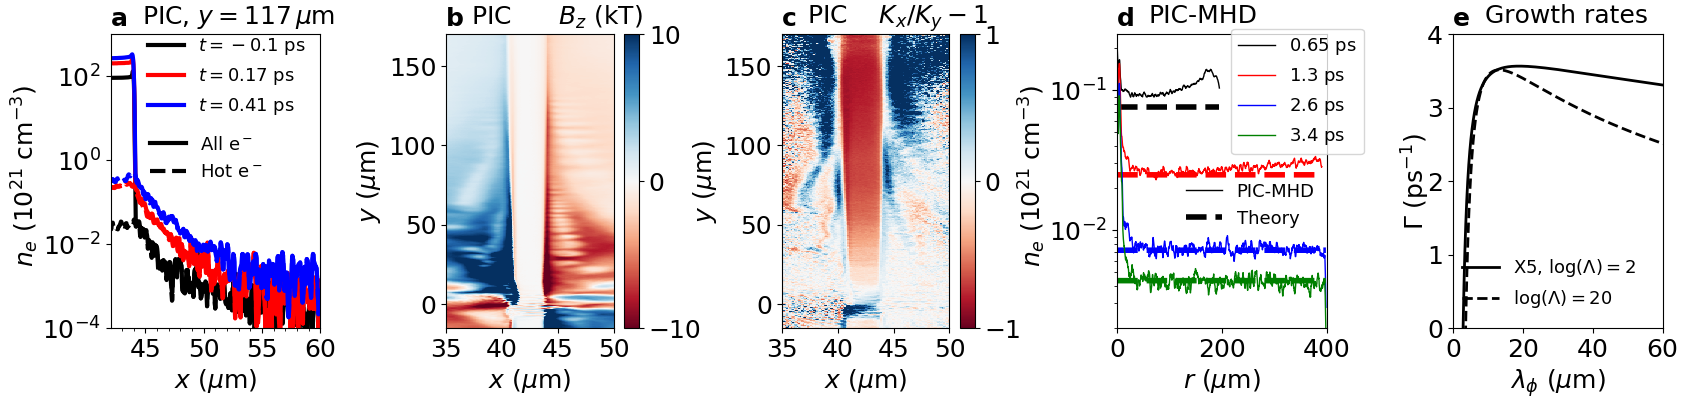
\includegraphics[scale=0.42]{Figure_3_new4.png}
\caption{\textcolor{blue}{
\textbf{Numerical simulation and theory of the current filamentation instabilities.}
{\bf a}-{\bf c}, Fully particle-in-cell (PIC), two-dimensional (2D)} simulation of the laser-plasma interaction in the $x-y$ plane (see Methods). 
{\bf a}, Longitudinal lineouts at $y=117\,\rm \mu m$ of the total (solid lines) and hot (kinetic energies $>100\,\rm eV$, dashed lines) electron density (in $10^{21}\,\rm cm^{-3}$ units) at different times, illustrating the hot-electron-driven plasma expansion along the target normal and away from the laser spot (located at $y=0$). In the expanding plasma ($x\gtrsim 44\,\rm \mu m$), the hot and total electron density profiles coincide.
{\bf b}, 2D map of the magnetostatic ($B_z$) field,  averaged over a laser cycle, at $t=0.41\,\rm ps$, showing magnetic modulations in the expanding plasma as the result of the collisionless Weibel instability.
{\bf c}, Electron momentum-flux anisotropy, $K_x/K_y-1$, where $K_x$ (resp. $K_y$) is the local $x$ (resp. $y$) aligned momentum flux, averaged over electrons of energies $>100\,\rm eV$.
{\bf d}, 2D PIC-MHD \textcolor{blue}{(particle-in-cell-magnetohydrodynamics)} simulation of hot-electron transport in the $y-z$ plane (see Methods) with $T_{h0}=1\,\rm MeV$, $n_{h0}=5 \times 10^{21}\,\rm cm^{-3}$, $R_0=32\,\rm \mu m$, $T_{c0}=50\,\rm eV$, and $\log \Lambda=2$. The hot-electron density $n_h/n_c$ (solid lines), averaged \textcolor{blue}{over the poloidal angle ($\phi = \tan^{-1}(y/z)$), is plotted vs. radius} $r=\sqrt{y^2+z^2}$ at different times, and compared with analytic estimates (dashed lines, see text).
\textbf{e}, Theoretical growth rate \textcolor{blue}{of the resistive current filamentation instability} $\Gamma$ vs. poloidal wavelength $\lambda_\phi$ (see Supplementary Information, Sec.~III). Hot-electron parameters are extracted \textcolor{blue}{at $t=1 \,\rm ps$} from PIC-MHD simulations run with $\log \Lambda = 2$, i.e., modeling a conductor (solid line, multiplied by 5 for clarity) and $\log \Lambda = 20$, i.e., modeling an insulator (dashed line), \textcolor{blue}{namely, $n_h \simeq 5\times 10^{19}\,\rm cm^{-3}$, $T_x \simeq 100\,\rm keV$, $T_c \simeq 200\,\rm eV$, $T_\phi = 3\,\rm keV$ (resp. $4\,\rm keV$) for $\log \Lambda =2$ (resp. 20)}  (see Methods).
}
\label{fig:pic}
\end{figure*}

We will now show that the recirculation of the hot electrons across the \textcolor{blue}{dilute} plasmas expanding from the target \textcolor{blue}{surfaces} triggers collisionless current filamentation, thus giving rise to electromagnetic structures such as those sketched in Fig.~\ref{fig:radio}e. In order to investigate the large-scale hot-electron dynamics in a self-consistent way, we have performed a 2D particle-in-cell (PIC) simulation using the code \textsc{calder} \cite{NF_Lefebvre_2003}. This simulation describes the laser-plasma interaction (and related collisional and ionization processes) in the $x-y$ plane shown in Fig.~\ref{fig:xp}, with half-reduced Al density to alleviate the computational effort (see Methods). Hereafter, the \textcolor{blue}{time origin is when} the pulse maximum reaches the target surface. We see in Fig.~\ref{fig:pic}a that, already at $t=0.41\, \rm ps$ (i.e., $1.44\,\rm ps$ \textcolor{blue}{after the start of the simulation}), the rear target surface has moved a distance $>10\,\rm \mu m$, and that magnetic modulations have developed in the expanding plasmas from the two target sides (see Fig.~\ref{fig:pic}b and Supplementary Figures 1 and 7). At the backside ($x>44\,\rm \mu m$), they extend up to $y \simeq 150\,\rm \mu m$ from the laser spot, with a typical wavelength $\lambda_p \simeq 6\,\rm \mu m$.

Electrons in the expanding \textcolor{blue}{plasmas} show a momentum-flux anisotropy $K_x/K_y - 1 \sim 1$ ($K_x$ and $K_y$ \textcolor{blue}{denote} the momentum fluxes along, respectively, the $x$ and $y$ directions, see Figs.~\ref{fig:pic}c and S1f), suggesting that they are susceptible to the Weibel filamentation instability~\cite{POP_Ren_2006, PRL_Gode_2017}. The growth rate \textcolor{blue}{($\Gamma_p$), wavelength ($\lambda_p$) and saturated field strength ($B_p$)} of the dominant mode \textcolor{blue}{have been} estimated from the dispersion relation derived for an \emph{ad hoc} two-temperature relativistic distribution function
(see Supplementary Information, Secs.~II \textcolor{blue}{and V.A}), the parameters of which \textcolor{blue}{being} extracted from the \textcolor{blue}{PIC} simulation. \textcolor{blue}{Introducing the hot-electron plasma frequency, $\omega_{ph}=\sqrt{n_h e^2/m_e \epsilon_0}$ and the electron \textcolor{blue}{(longitudinal)} thermal velocity $v_{hx}$, $\lambda_p$ and $B_p$ can be expressed as}
\begin{align}
  \lambda_p &\simeq 2\pi \alpha_\lambda c/\omega_{ph} \label{eq:lp} \,,\\
  B_p &\simeq \alpha_\Gamma^2\alpha_\lambda m_e \omega_{ph}c/ev_{hx} \label{eq:bp} \,, 
\end{align}
where $c$, $\epsilon_0$, $n_h$, $m_e$ and $e$ are the speed of light in vacuum, the vacuum permittivity, the hot electron density, the electron mass and charge, respectively. \textcolor{blue}{The proportionality factors $\alpha_\lambda$ and $\alpha_\Gamma$ depend} on the anisotropy and mean energy of the electron distribution \textcolor{blue}{(see Supplementary Figure 4)}. In our case, we have \textcolor{blue}{typically $\alpha_\lambda \sim 2$, $\alpha_\Gamma \sim 0.1$ and $v_{hx} \sim 0.5 c$}.

In order to demonstrate that the instability seen to grow in the simulated expanding \textcolor{blue}{plasmas} (Fig.~\ref{fig:pic}b) accounts for the dotted pattern evidenced by the radiographs (Fig.~\ref{fig:radio}), one needs to disentangle the impact of the reduced simulation geometry on the hot-electron dynamics. Indeed, unlike in Refs.~\cite{PRL_Gode_2017, NJP_Scott_2017}, field modulations here build up at least a picosecond after laser irradiation, and hundreds of microns away from the focal spot, where multidimensional electron dilution effects should arise. Obviously, such effects are improperly treated in our fully PIC 2D simulation, which resolves only the $x-y$ plane. Yet they can be evaluated by estimating the temporal evolution of the hot-electron density, $n_h$, in a general system of spatial dimension $D+\delta$, where $D$ and $\delta$ denote the \textcolor{blue}{degrees of freedom} in the target plane and normally to it, respectively. Assuming a homogeneous spatial distribution, and taking into account \textcolor{blue}{the expansion of the hot electrons in both the transverse and longitudinal directions},
one obtains \textcolor{blue}{$n_h(t) \simeq \alpha_n n_{h0}(1+ v_{hr} t /R_0)^{-D}(1+ 2c_{sh} t/L)^{-\delta}$} with $L$, $R_0$, $n_{h0}$, $\alpha_n$, $v_{hr}$, and $c_{sh}$ being the initial target thickness, hot-electron source radius, initial hot-electron density, \textcolor{blue}{fraction} of spreading hot electrons, effective radial velocity and sound velocity. Our fully PIC simulation \textcolor{blue}{indicates that} $R_0 \simeq 32\,\rm \mu m$ and $n_{h0} \simeq 5\times 10^{21}\,\rm cm^{-3}$ (see Supplementary Figure 3a).

To constrain the above values of $\alpha_n$ and $v_{hr}$, we have carried out a 2D PIC-MHD simulation resolving the hot-electron transport through the solid-density Al target in the transverse ($y-z$) plane. In this simulation, the laser-plasma interaction and longitudinal plasma expansion are not described, while the response of the thermal bulk electrons is modeled in the resistive MHD limit, which allows the hot electrons to be followed over larger spatiotemporal scales than in the fully PIC simulation (see Methods). At $t=0$, the hot electrons are initialized as an isotropic Maxwellian population of temperature $T_{h0}=1\,\rm MeV$ and density $n_{h0}=5\times10^{21}\,\rm cm^{-3}$, contained in a circular region of radius $R_0=32\,\rm \mu m$. The initial Al plasma temperature is of $50\,\rm eV$, corresponding to a $5+$ ionization degree. \textcolor{blue}{These} input parameters are based on the fully PIC simulation data (see Supplementary Information, Sec.~I).

The hot-electron density profiles extracted at various times from the PIC-MHD simulation (see Figs.~\ref{fig:pic}d and S7) support the above estimate for $n_h(t)$, with $D=2$, $\delta=0$, $\alpha_n \simeq 0.25$ and $v_{hr}\simeq 0.5c$ (see Supplementary Information, Sec.~IV.B). Also, taking $D=\delta=1$, our formula predicts \textcolor{blue}{$n_h \simeq 1 \times 10^{20}\,\rm cm^{-3}$ at $t\simeq 0.4\,\rm ps$}, consistent with the fully PIC simulation (Fig.~\ref{fig:pic}a). Further, Eqs.~\eqref{eq:lp} and \eqref{eq:bp} \textcolor{blue}{give $\lambda_p \simeq 7\,\rm \mu m$ and $B_p \simeq 120\,\rm T$}, close to the simulation data (see Fig.~\ref{fig:pic}b and Supplementary Figure 1b). 

In the experimental geometry ($D=2$, $\delta=1$), \textcolor{blue}{assuming $T_h \simeq 100\,\rm keV$ (as estimated at $\gtrsim 100\,\rm \mu m$ distances from the source, see Supplementary Figure 6 and Sec.~IV.A), one obtains $n_h \simeq 3 \times 10^{17}\,\rm cm^{-3}$ at $t=4\,\rm ps$, which translates into a growth time $\Gamma_p^{-1} \simeq 0.3\,\rm ps$ and a typical wavelength  $\lambda_p \simeq 110\,\rm \mu m$, in fair agreement with the rapid development and size of the observed structures (Figs.~\ref{fig:radio}a-c).
A magnetic field strength $B_p \simeq 7\,\rm T$ is also predicted, comparable with the experimentally inferred value of $\sim 5\,\rm T$ (see Methods). Note that the electric fields accompanying the magnetic modulations \cite{POP_Dieckmann_2009, POP_Bret_Gremillet_2010} should only weakly affect the radiographs (see Supplementary Information, Sec.~V.B).} Since hot-electron recirculation and target expansion occur on both \textcolor{blue}{target sides}, the \textcolor{blue}{probe} protons should form two overlaid, independent \textcolor{blue}{modulation} patterns on the detector (see Methods and Supplementary Information, Sec.~V.C).

\begin{figure*}
%\centerline{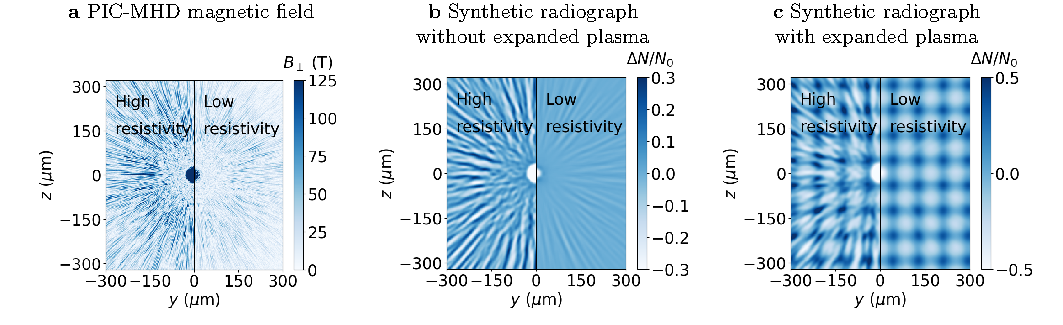
\includegraphics[scale=0.99]{Fig4.pdf}}
\caption{\textcolor{blue}{
\textbf{PIC-MHD simulations of the resistive filamentation and synthetic radiographs.}
\textbf{a}, Spatial distribution of} $B_\perp=(B_y^2+B_z^2)^{1/2}$ (in Teslas) at time $t=3.28\,\rm ps$ for $\log \Lambda=20$ (i.e., modeling an insulator, $y<0$) and $\log\Lambda=2$ (i.e., modeling a conductor, $y>0$).
\textbf{b}, Synthetic radiographs from $8\,\rm MeV$ \textcolor{blue}{probe} protons of a 
$3\,\rm \mu m$ thick target with $B$-fields given by \textbf{a} (see Methods).
\textbf{c}, Synthetic radiographs with superimposed filaments extending in $x$ direction over $L_p=48\,\rm \mu m$ (see Methods).
Following Fig.~\ref{fig:radio}e, \textcolor{blue}{the electromagnetic fields used for the reconstruction are taken to obey the radial profiles given by Eqs.~\eqref{eq:bloop} and \eqref{eq:eloop}, with $B_0=5\,\rm T$ and $a=30\,\rm \mu m$, together with a periodicity $\lambda_p=120\,\rm \mu m$.}
%be poloidal around each filament center (of periodicity $\lambda_p=120\,\rm \mu m$), 
One electromagnetic distribution has been placed on the expanding rear side of the target (see Methods for details on their arrangement) }
\label{fig:kxy}
\end{figure*}

The PIC-MHD simulations capture the lateral spreading dynamics of the hot electrons, and hence the resistive filamentation instability that \textcolor{blue}{they can drive}. As the electrons move radially away from their generation region, their momentum distribution becomes \textcolor{blue}{``colder'' in the poloidal ($\phi$) direction than in the other ($r,x$) directions (see Supplementary Figure 6 and Sec.~IV.A). In particular, a large momentum flux anisotropy arises in the $x-\phi$ plane} in $\sim 0.5\,\rm ps$, although its final level may be overestimated due to neglect of the longitudinal target expansion and of the associated electron-to-ion momentum transfer (occurring after $\sim L/2c_{sh} \sim 0.5\,\rm ps$ \cite{PRE_Mora_2005}). Therefore, in the case of the conducting Al target (characterized by a Coulomb logarithm $\log \Lambda = 2$~\cite{POF_Lee_1984}), a non-propagating (in-plane) magnetic modulation builds up after a few $100\,\rm fs$ (see \mbox{Fig.~\ref{fig:kxy}a, right}), reaching a strength $\langle B_\phi^2\rangle^{1/2}\simeq 34\,\rm T$ (averaged over the region $100 \le r \le 200\,\mu \rm m$) with a typical (poloidal) wavelength $\lambda_\phi \simeq 5-10\,\rm \mu m$. These results are compatible with the linear dispersion relation of the resistive filamentation instability, evaluated using parameters extracted from the PIC-MHD simulation at $t=1\,\rm ps$, and \textcolor{blue}{predicting} a fastest-growing wavelength $\lambda_\phi \simeq 10\,\mu \rm m$ (see Fig.~\ref{fig:pic}e and Methods). 

\textcolor{blue}{Let us} now assess the influence of the target electrical resistivity on the observed radial structures. The hot-electron dynamics in the insulating PET target is expected to differ from that in the conducting Al target due to a higher electrical resistivity at low temperatures \cite{PRL_Fuchs_2003, PRL_McKenna_2011}. Since our PIC-MHD framework ceases to be accurate outside the Spitzer collisional regime ($T\lesssim 50\,\rm eV$), we restrict ourselves to a qualitative comparison by running the same simulation than in Al but with an artificially enhanced resistivity, i.e., using a Coulomb logarithm $\log \Lambda = 20$ instead of $\log \Lambda = 2$, so as to mimic the response of the PET bulk electrons. Comparing the magnetic field maps displayed in the left and right-hand sides of Fig.~\ref{fig:kxy}a, about twice stronger field modulations ($\langle B_\phi^2 \rangle^{1/2} \simeq 70\,\rm T$ vs. $35\,\rm T$) \textcolor{blue}{have arisen} at $\log \Lambda = 20$, while keeping approximately the same wavelength. This behavior \textcolor{blue}{matches the expected properties}
of the resistive filamentation instability (see Methods and Supplementary Information, Sec.~III). Indeed, from the simulation data in the region $50 \le r \le 100\,\rm \mu m$ (see Supplementary Figure 6), the maximum growth rate (dashed line in Fig.~\ref{fig:pic}e) is predicted to be \textcolor{blue}{$\sim 5$} times larger at $\log \Lambda = 20$ than at $\log \Lambda = 2$, \textcolor{blue}{yet} with about the same wavelength. \textcolor{blue}{The resistive filamentation growth time, $\Gamma^{-1} \simeq 0.3\,\rm ps$, turns out to be similar to that of the collisionless instability, and compatible with the experimental time of appearance of the proton dose modulations.} 

After saturation of the instability, the hot electrons' contribution to the magnetic structures progressively weaken due to dilution, so that the latter end up being sustained by the bulk thermal electrons only, thus being subject to magnetic diffusion over a timescale $\tau_d \simeq \mu_0 \sigma \lambda_\phi^2 \gtrsim 30\,\rm ps$ at temperatures $\gtrsim 50\,\rm eV$. Hence, we do not expect significant evolution of the fields inside the target over a $\sim \tau_d$ timescale following the final simulation time ($3.28\,\rm ps$).

Figures~\ref{fig:kxy}b,c display synthetic radiographs obtained from proton ray-tracing through the field distributions \textcolor{blue}{provided by} the above simulations (see Methods). In Fig.~\ref{fig:kxy}b only the PIC-MHD fields are taken into account (for both $\log \Lambda =2$ and $\log \Lambda = 20$), while Fig.~\ref{fig:kxy}c further considers the effect of the electric and magnetic fluctuations \textcolor{blue}{generated} in the expanding \textcolor{blue}{plasmas}. In all cases, \textcolor{blue}{collisional} scattering of the \textcolor{blue}{probe} protons is also described (see Methods), \textcolor{blue}{causing} the smoothed rendering of Fig.~\ref{fig:kxy}b compared to Fig.~\ref{fig:kxy}a. In the low-resistivity (Al) target,  Figs.~\ref{fig:kxy}b,c show that the dotted field pattern in the expanding \textcolor{blue}{plasmas} mainly accounts for the observed proton modulations. In the high-resistivity (PET) target, by contrast, \textcolor{blue}{those modulations result from the field fluctuations generated in both the expanding plasmas and the bulk target}. The larger number of radial structures in the synthetic radiographs (Figs.~\ref{fig:radio}f,g) is ascribed to the imperfect modeling of the electrical resistivity of the target and to uncertainties in the initial hot-electron parameters.

A full quantitative understanding of our experimental observations would require \textcolor{blue}{the multidimensional hot-electron kinetics in dense plasmas to be described} over tens of ps and hundreds of $\rm \mu m$ spatiotemporal scales. Not only out of reach of state-of-the-art kinetic simulation codes, this challenging problem also implies progress in the theoretical modeling of the coupled-to-weakly-coupled plasma transition during laser irradiation.


\section*{Methods}
\subsection*{Experiments}

The experiment was performed at the Jupiter Laser Facility's \textsc{titan} laser at the Lawrence Livermore National Laboratory \cite{RSI_Albertazzi_2015}. Each laser beam B1 and B2 had an energy of $55\,\rm J$ ($\pm 10\%$), a pulse duration of $\sim 700\,\rm fs$ FWHM, and was focused with a $f/3$ parabola at $31^\circ$ incidence angle in the horizontal plane, resulting in an on-target intensity of $\sim 2\times 10^{19}\,\rm W.cm^{-2}$. The normalized laser field strength was $a_L \equiv eE_L/m_e c\omega_L \simeq 4$ ($E_L$ and $\omega_L$ are the laser electric field strength and frequency). Before focusing, B1 was reflected off a plasma mirror, with $70\,\%$ efficiency, in order to improve its temporal contrast \cite{PRE_Doumy_2004}. A high temporal contrast ensured steep density gradients at the target surface, which is critical for the formation and observation of the far-distant magnetic loop structures revealed here (e.g., compare with the results of Ref.~\cite{PRL_Sarri_2012} where no similar structures were observed, likely due to the generation of a large preplasma by the laser prepulse). 
The probe protons, generated through target normal sheath acceleration \cite{PRL_Fuchs_2003} by focusing B2 onto a $50\,\rm \mu m$-thick Au foil, had a useful energy range of $4.5\,\rm MeV$ to $9.5\,\rm MeV$. They probed the $B$-fields developing in target 1 in a ``face-on'' configuration \cite{RSI_Albertazzi_2015}, suited to measuring toroidal magnetic loops having their axis along the target normal, while minimizing the influence of the $E$-fields that develop along the target normal. As shown in Fig.~\ref{fig:xp}, the probe protons, after propagation through target 1, were collected by a stack of radiochromic films \textcolor{blue}{(placed 39 mm behind target 1)} in which they were stopped in distinct layers according to their incident energy \cite{RSI_Chen_2016}. Time-of-flight differences between protons of various energies from their source up to target 1 allowed us to probe the central, large-scale, as well as the radially distant, smaller-scale, electromagnetic fields at successive times ($t=0$ corresponds to the time at which B1 strikes target 1). Target 1 was either a $3\,\rm \mu m$-thick Aluminum (Al) foil or a $10\,\rm \mu m$-thick Polyethylene terephthalate [PET, an insulator polymer with composition $(\mathrm{C}_{10}\mathrm{H}_8\mathrm{O}_4)_n$].
 
\subsection*{2D fully PIC simulation}

A large-scale PIC simulation (2D in space, 3D in momentum) of the irradiation of the Al foil by the laser beam \textcolor{blue}{B1} has been performed using the PIC code \textsc{calder} \cite{NF_Lefebvre_2003}. The laser beam has a Gaussian temporal profile of $690\,\rm fs$ FWHM, a Gaussian spatial profile of $8\,\rm \mu m$ FWHM and a $30^\circ$ incidence angle. Its maximum intensity is of $3.5 \times 10^{19}\,\rm W.cm^{-2}$, reached at $t=0\,\rm ps$ on the target surface. The simulation \textcolor{blue}{is run from $t = -1.03\,\rm ps$ to} $t = 0.41\,\rm ps$. The target is composed of three layers: H$^+$ ($0.7\,\rm \mu m$), Al$^{3+}$ ($3.7\,\rm \mu m$) and neutral hydrogen ($6\,\rm nm$). Its density profile consists of a $3\,\rm \mu m$ long plateau preceded by a $1.4\,\rm \mu m$-long preplasma made of H$^+$ and Al$^{3+}$ ions. The maximum ion target density is taken to be half the solid density ($n_\mathrm{Al}=n_\mathrm{H}=90 n_c$) so as to reduce the computational load. All species are initialized with a temperature of $10\,\rm eV$.

The numerical box has dimensions $L_x \times L_y = 83.5 \times 389.9\,\rm \mu m^2$ with a spatial discretization $\Delta x = \Delta y = 5.6\,\rm nm$ and a time step $\Delta t = 1.48\times 10^{-2}\,\rm fs$. An alternating-order interpolation scheme \cite{CPC_Sokolov_2013} is employed with a 4th-order weight factor. Each cell initially contains 50 macroparticles per species in the Al layer and 500 macroparticles per species in the thin H layers. The Maxwell solver proposed in Ref.~\cite{PRSTAB_Lehe_2013} is used along with a combination of spatial \cite{JCP_Vay_2011} and temporal \cite{JCP_Friedman_1990} filtering. Elastic Coulomb collisions, electron impact ionization and field ionization are modeled following Refs.~\cite{POP_Perez_2012}.

\subsection*{2D PIC-MHD simulations}

In order to access spatiotemporal scales of experimental relevance in a 2D geometry, we have employed the resistive magnetohydrodynamic (MHD) PIC model proposed in Ref.~\cite{JCP_Cohen_2010}. This numerical scheme, implemented into the code \textsc{calder} \cite{NF_Lefebvre_2003}, consists in replacing the Maxwell-Amp\`ere equation with the generalized Ohm's law
\begin{equation} \label{eq:PICMHD}
  \mathbf{E}=\eta \left(\nabla \times \mathbf{B}-\mathbf{j}_h-\frac{\partial \mathbf{E}}{\partial t}\right)+\frac{\mathbf{j}_c\times \mathbf{B}}{en_c}
  -\frac{\nabla P_c}{en_c} \,,
\end{equation}
where $\eta$ is the electrical resistivity, $n_c$, $P_c$ and $\mathbf{j}_c$ are the density, pressure and current density of the thermal (`cold' or `bulk') electrons and $\mathbf{j}_h$ is the current density of the hot electrons. Since this scheme only accounts for the generation of nonradiative fields, it allows one to use mesh sizes (resp. time steps) much larger than the plasma skin depth (resp. plasma period), thus greatly alleviating the computational load. In a given cell, electrons are considered `cold' if their velocity fulfills $v<5\sqrt{T_c/m_e}$, where $T_c$ is the local temperature of the cold electron population at the previous time step; the remaining electrons are considered `hot'.

The PIC-MHD simulations (2D in configuration space and 3D in momentum space) describe the self-consistent evolution of an initially confined source of hot electrons through a dense Al plasma in the $y-z$ plane parallel to the target surface (assuming invariance along the $x$ axis). Initially, the hot electrons uniformly fill a cylinder of radius $R_0=32\,\rm \mu m$ with a density $n_{h0}=5\times 10^{21}\,\rm cm^{-3}$, centered around $(y,z)=(0,0)$. The start time of the simulation ($t=0$) is assumed to correspond approximately to the moment when the maximum laser intensity reaches the target surface, thus reducing the time-dependent hot-electron generation to a instantaneous process. The choice of an initial hot-electron source wider than the $\sim 8\,\rm \mu m$ laser spot partly accounts for the radial expansion of the hot electrons during the laser pulse \cite{PRE_Stephens_2004} (thus ensuring a relatively moderate $n_{h0}$, as is expected). Their momenta are distributed according to an isotropic Maxwell-J\"uttner distribution of temperature $T_{h0}=1\,\rm MeV$. Simulations performed with different initial \textcolor{blue}{hot-electron} temperatures (from $200$ to $700\,\rm keV$) or anisotropic distributions (with $T_x>T_{y,z}$) yield qualitatively similar results. The total kinetic energy carried by the hot electrons is $\sim 25\,\rm J$, which amounts to $\sim 50\%$ of the \textcolor{blue}{B1} laser energy \cite{PRL_Ping_2008}. The hot-electron spot is immersed inside a solid-density Al$^{5+}$ plasma of \mbox{50~eV} temperature. The bulk electron density is $n_{c0}=300n_c$ everywhere, except within the hot spot, where it reduces to $n_{c0}=295n_c$ to ensure charge neutrality. Coulomb binary collisions between all charged particle species and impact ionization of the Al ions are described using the framework of Ref.~\cite{POP_Perez_2012}. The electrical resistivity involved in Ohm's law is calculated in the Spitzer regime with the numerical fits given in Ref.~\cite{Decoster_1998}. 
The computational domain has dimensions $L_x\times L_y=800 \times 800\,\rm \mu m^2$ and is discretized with mesh sizes $\Delta x=\Delta y =0.16\,\rm \mu m$. The time step is $\Delta t=0.34\,\rm fs$. The boundary conditions are taken to be absorbing for the particles and reflective for the fields. The ion and cold electron populations are initially modeled by 100 macroparticles per cell, while the hot electrons are modeled by 1000 macroparticles per cell. 

\subsection*{Theory of the resistive filamentation instability}

The dispersion relation of the filamentation instability driven by hot electrons streaming through a dense resistive plasma has been derived within a kinetic-fluid framework, similarly to Ref.~\cite{POP_Gremillet_2002}. The hot electrons are \textcolor{blue}{assumed} to obey a multi-temperature Maxwellian distribution (neglecting relativistic effects, \textcolor{blue}{as is justified at ps time scales and far from the laser spot}), and their perturbed current density is obtained from the linearized Vlasov equation. The bulk electron current is given by the simple Ohm's law $\mathbf{j}_c=\sigma \mathbf{E}$.
\textcolor{blue}{A third-order Taylor expansion of the dispersion relation allows the instability growth rate to be analytically solved as a function of the poloidal} fluctuation wavenumber (see Supplementary Information, \textcolor{blue}{Sec.~III}). The input electron parameters \textcolor{blue}{for the growth rate curves plotted in Fig.~\ref{fig:pic}e} have been extracted from PIC-MHD simulations \textcolor{blue}{run with $\log \Lambda = 2$ (Fig.~\ref{fig:kxy}a, right) and $\log \Lambda=20$ (Fig.~\ref{fig:kxy}a, left).} The hot-electron density ($n_h$), \textcolor{blue}{longitudinal temperature ($T_x$) and poloidal temperature ($T_\phi$) are taken to be $n_h=5\times 10^{19}\,\rm cm^{-3}$, $T_x=100\,\rm keV$, and $T_\phi=3\,\rm keV$ (resp. $T_\phi = 4\,\rm keV$) for $\log \Lambda=2$ (resp. $\log \Lambda=20$), see Supplementary Figure 6. The bulk electron temperature is set to $T_c=200\,\rm eV$ in both cases. Variations in those parameters over the ranges observed in the simulations at $\gtrsim 100\,\rm \mu m$ radii may alter the shape and level of the low- and high-resistivity curves (solid and dashed lines in Fig.~\ref{fig:pic}e), yet without changing their ordering}

\subsection*{Synthetic proton radiographs}

The synthetic proton radiographs displayed in Fig.~\ref{fig:kxy} have been generated using the \textsc{ilz} program developed at LULI. This numerical tool allows us to confront the kinetic simulation results with the experimental data (Fig.~\ref{fig:radio}), and hence to infer the topology of the proton-probed magnetic fields.

\textsc{ilz} computes numerically the proton trajectories in a given stationary electromagnetic distribution, neglecting collective effects. 
The input proton flux is taken to be monoenergetic with a uniform angular distribution within an emission lobe broad enough  ($>8^\circ$) to probe the whole PIC-MHD simulation plane. The dose variation onto the detector plane is evaluated as $\Delta N/N_0= (N-N_0)/N_0$, where $N_0$ and $N$ are the locally measured fluxes (in a given solid angle) before and after crossing the electromagnetic distribution. Owing to the small areal density of the target, the collisional energy loss of the protons can be neglected. Their collisional angular scattering is modeled by convolving the dose variation with a Gaussian \textcolor{blue}{corresponding to an rms angular width} \cite{NIM_Highland_1975}:
\begin{equation}
\theta_{1/e}  = \frac{E_s}{p\beta c} \sqrt{\frac{L}{L_R}} \epsilon \,,
\end{equation}
where $L$ is the target thickness, $L_R$ is the radiation length of the material, $p$ is the incident proton momentum, $\epsilon = 1 + 0.038 \log\left(L/L_R\right)$ is a correction term~\cite{EPJ_Groom_2000}, and $E_s=13.6\,\rm MeV$ is a constant.
\textcolor{blue}{One has $\theta_{1/e}  = 4.24\,\rm mrad$ and $3.70\,\rm mrad$ in the aluminum and PET targets, respectively.}

\textcolor{blue}{The magnetic field distribution is taken in the form of a periodic array of magnetic loops with interspacing $\lambda_p$. The azimuthal magnetic field within each elementary structure has the following radial profile,
\begin{equation}\label{eq:bloop}
B_\theta(r) = \pm \sqrt{2 e_N} B_0 \frac{r}{a} e^{-r^2/a^2} \,,
\end{equation}}
with $a$ being the radial size of the structure, $B_0$ its maximum field strength \textcolor{blue}{and $e_N \equiv \exp(1)$. The magnetic field distribution is assumed to comprise magnetic loops of opposite polarity, as drawn in Fig.~\ref{fig:radio}e (the colormap depicts the \textsc{ilz}-computed proton dose variations).}

The electric field \textcolor{blue}{within each magnetic loop} has been estimated by balancing its resulting force on the plasma electrons and the magnetic pressure force, giving $E_r = -\nabla B^2 /(2\mu_0e n_h)$~\cite{POP_Dieckmann_2009, POP_Bret_Gremillet_2010}. 
\textcolor{blue}{Using Eq.~\eqref{eq:bloop} leads to
\begin{equation}\label{eq:eloop}
E_r(r) = -
\frac{4}{\pi^2\alpha_\lambda^2}
\frac{2e_N e B_0^2}{m_e} r\left( 1-\frac{2r^2}{a^2}\right) e^{-2r^2/a^2} \,.
\end{equation}
While the filament radius $a$ could be related to the hot-electron density (through $a \simeq \lambda_p/4=\pi \alpha_\lambda c/2\omega_{ph}$), we have considered it as a fitting parameter, together with the field strength $B_0$.}

The modulations \textcolor{blue}{in} the proton dose deposited in the RCF have been evaluated using the calibration performed in Ref.~\cite{RSI_Chen_2016}. The reference dose (from the non-deflected protons) \textcolor{blue}{was} measured outside of the modulated area. The field parameters \textcolor{blue}{$B_0$ and $a$ were inferred by fitting the data to the synthetic dose modulations.} Figure~\ref{fig:radio}d illustrates this procedure in the Al case: the two locally best-matching synthetic dose profiles, corresponding to \textcolor{blue}{$(B_0,a)=(5.2\,\rm T, 30\,\rm \mu m)$} (black dashed line) and \textcolor{blue}{$(B_0,a)=(3\,\rm T,18\,\rm \mu m)$} (blue dashed line), are overlaid on the experimental profile (purple solid line). Figure~\ref{fig:radio}h exemplifies the PET case: here the \textcolor{blue}{streak-like dose modulations due to the resistive instability (red solid line) are well reproduced assuming magnetic filaments of $\sim 33\,\rm \mu m$ FWHM and $\sim 40\,\rm T$ amplitude (black dashed line).}

The electromagnetic field distribution underpinning the synthetic proton images shown in Fig.~\ref{fig:kxy}c consists of the juxtaposition of \textcolor{blue}{the above-discussed} electromagnetic loops (placed at the rear side of the target) and the electromagnetic field map extracted from the PIC-MHD simulation. In other terms, in the \textsc{ilz} simulation, the protons first probe the fields predicted by the PIC-MHD simulation, and then the electromagnetic loops formed in the expanding plasma at the target backside. \textcolor{blue}{The periodicity of the field structures and the thickness of the expanding plasma have been set to $\lambda_p=120\,\rm \mu m$ and $L_p \simeq c_{sh}t \simeq 48\,\rm \mu m$ ($t\simeq 4\,\rm ps$ is the probing time). For completeness, synthetic radiographs obtained by placing electromagnetic loops on both target sides are displayed} in Supplementary Figure 10. 

\begin{acknowledgments}
The authors gratefully acknowledge F.~Amiranoff, F.~Fiuza, E.~d'Humi\`eres, V.~Gubchenko, and V.T.~Tikhonchuk for insightful discussions.
They also acknowledge the support of the JLF-Titan technical teams.
The simulations were performed using HPC resources at TGCC/CCRT. We acknowledge PRACE for awarding us access to TGCC/Curie (Grant No. 2014112576).
This project has received funding from the European Union’s Horizon 2020 research and innovation program under grant agreement no 654148 Laserlab-Europe and from the European Research Council (ERC) under the European Union’s Horizon 2020 research and innovation programme (grant agreement No 787539).
The research leading to these results is supported by Extreme Light Infrastructure Nuclear Physics (ELI-NP) Phase II, a project co-financed by the Romanian Government and European Union through the European Regional Development Fund. This work was partly done within the LABEX Plas@Par project. It was supported by Grants No. 11-IDEX-0004-02 and ANR-17-CE30-0026-Pinnacle from Agence Nationale de la Recherche. This work was also partly supported by the DFG GRK 1203 and SFB/TR18 programs and by EPSRC grants EP/K022415/1 \& EP/J002550/1.
This work was supported in part by the Ministry of Education and Science of the Russian Federation under Contract No.14.Z50.31.0007.
The use of the Jupiter Laser Facility  was supported by the U.S. Department of Energy, Lawrence Livermore  National Laboratory, under Contract No. DE-AC52-07NA27344.
\end{acknowledgments}

\section*{Author contributions}
JF conceived the project. BA, SNC, PA, JB, VD, LL, MN, LR, MSw, MB, HP and JF performed the experiment, with support from RS, OW and MSt.  BA, SB and JF analyzed the data. CRu and LG developed the theoretical framework and performed the simulations, with discussions with MG and CRi. SB computed the synthetic proton radiographs. JF, CRu and LG wrote the paper. All authors commented on the paper at its various stages.

\section*{Competing interests}
The authors declare no competing interests. 

\section*{Data availability}
The data that support the findings of this study are available from the corresponding authors upon reasonable request. 

\section*{Code availability}
The codes that support the findings of this study are available from the corresponding authors upon reasonable request.

%\bibliographystyle{naturemag}
%\bibliography{biblio}
\begin{thebibliography}{10}
\expandafter\ifx\csname url\endcsname\relax
  \def\url#1{\texttt{#1}}\fi
\expandafter\ifx\csname urlprefix\endcsname\relax\def\urlprefix{URL }\fi
\providecommand{\bibinfo}[2]{#2}
\providecommand{\eprint}[2][]{\url{#2}}

\bibitem{Shkarofsky_1966}
\bibinfo{author}{Shkarofsky, I.}, \bibinfo{author}{Johnston, T.} \&
  \bibinfo{author}{Bachynski, M.}
\newblock \emph{\bibinfo{title}{The particle kinetics of plasmas}}
  (\bibinfo{publisher}{Addison-Wesley Pub. Co.}, \bibinfo{year}{1966}).

\bibitem{Belmont_2013}
\bibinfo{author}{{Belmont}, G.}, \bibinfo{author}{Roland, G.},
  \bibinfo{author}{Mottez, F.}, \bibinfo{author}{Pantellini, F.} \&
  \bibinfo{author}{Pelletier, G.}
\newblock \emph{\bibinfo{title}{{Collisionsless plasmas in astrophysics}}}
  (\bibinfo{publisher}{Wiley}, \bibinfo{year}{2013}).

\bibitem{Davidson_1983}
\bibinfo{author}{Davidson, R.~C.}
\newblock \bibinfo{title}{Kinetic waves and instabilities in uniform plasmas}.
\newblock In \bibinfo{editor}{Rosenbluth, M.~N.} \& \bibinfo{editor}{Galeev, R.~Z.} (eds.) \emph{\bibinfo{booktitle}{{Handbook of Plasma Physics}}},
  vol.~\bibinfo{volume}{1} (\bibinfo{publisher}{North-Holland},
  \bibinfo{address}{Amsterdam}, \bibinfo{year}{1983}).

\bibitem{PRL_Weibel_1959}
\bibinfo{author}{Weibel, E.~S.}
\newblock \bibinfo{title}{Spontaneous growing transverse waves in a plasma due to an anisotropic velocity distribution}.
\newblock \emph{\bibinfo{journal}{Phys. Rev. Lett.}}
  \textbf{\bibinfo{volume}{2}}, \bibinfo{pages}{83--84} (\bibinfo{year}{1959}).

\bibitem{POF_Fried_1959}
\bibinfo{author}{Fried, B.~D.}
\newblock \bibinfo{title}{Mechanism for instability of transverse plasma waves}.
\newblock \emph{\bibinfo{journal}{Phys. Fluids}} \textbf{\bibinfo{volume}{2}},
  \bibinfo{pages}{337--337} (\bibinfo{year}{1959}).

\bibitem{POF_Davidson_1972}
\bibinfo{author}{Davidson, R.~C.}, \bibinfo{author}{Hammer, D.~A.},
  \bibinfo{author}{Haber, I.} \& \bibinfo{author}{Wagner, C.~E.}
\newblock \bibinfo{title}{Nonlinear development of electromagnetic instabilities in anisotropic plasmas}.
\newblock \emph{\bibinfo{journal}{Phys. Fluids}} \textbf{\bibinfo{volume}{15}},
  \bibinfo{pages}{317--333} (\bibinfo{year}{1972}).

\bibitem{PRL_Lee_1973}
\bibinfo{author}{{Lee}, R.} \& \bibinfo{author}{{Lampe}, M.}
\newblock \bibinfo{title}{{Electromagnetic instabilities, filamentation, and focusing of relativistic electron beams}}.
\newblock \emph{\bibinfo{journal}{Phys. Rev. Lett.}}
  \textbf{\bibinfo{volume}{31}}, \bibinfo{pages}{1390--1393}
  (\bibinfo{year}{1973}).

\bibitem{PRL_Adam_2006}
\bibinfo{author}{Adam, J.~C.}, \bibinfo{author}{H\'{e}ron, A.} \&
  \bibinfo{author}{Laval, G.}
\newblock \bibinfo{title}{Dispersion and transport of energetic particles due to the interaction of intense laser pulses with overdense plasmas}.
\newblock \emph{\bibinfo{journal}{Phys. Rev. Lett.}}
  \textbf{\bibinfo{volume}{97}}, \bibinfo{pages}{205006}
  (\bibinfo{year}{2006}).

\bibitem{RPP_Marcowith_2016}
\bibinfo{author}{{Marcowith}, A.} \emph{et~al.}
\newblock \bibinfo{title}{{The microphysics of collisionless shock waves}}.
\newblock \emph{\bibinfo{journal}{Rept. Prog. Phys.}}
  \textbf{\bibinfo{volume}{79}}, \bibinfo{pages}{046901}
  (\bibinfo{year}{2016}).

\bibitem{APJ_Schlickeiser_2003}
\bibinfo{author}{{Schlickeiser}, R.} \& \bibinfo{author}{{Shukla}, P.~K.}
\newblock \bibinfo{title}{{Cosmological magnetic field generation by the Weibel instability}}.
\newblock \emph{\bibinfo{journal}{Astrophys. J. Lett.}}
  \textbf{\bibinfo{volume}{599}}, \bibinfo{pages}{L57--L60}
  (\bibinfo{year}{2003}).

\bibitem{PRL_Allen_2012}
\bibinfo{author}{Allen, B.} \emph{et~al.}
\newblock \bibinfo{title}{Experimental study of current filamentation instability}.
\newblock \emph{\bibinfo{journal}{Phys. Rev. Lett.}}
  \textbf{\bibinfo{volume}{109}}, \bibinfo{pages}{185007}
  (\bibinfo{year}{2012}).

\bibitem{PRL_Fox_2013}
\bibinfo{author}{Fox, W.} \emph{et~al.}
\newblock \bibinfo{title}{Filamentation instability of counterstreaming laser-driven plasmas}.
\newblock \emph{\bibinfo{journal}{Phys. Rev. Lett.}}
  \textbf{\bibinfo{volume}{111}}, \bibinfo{pages}{225002}
  (\bibinfo{year}{2013}).

\bibitem{NP_Huntington_2015}
\bibinfo{author}{Huntington, C.~M.} \emph{et~al.}
\newblock \bibinfo{title}{Observation of magnetic field generation via the {Weibel} instability in interpenetrating plasma flows}.
\newblock \emph{\bibinfo{journal}{Nat. Phys.}} \textbf{\bibinfo{volume}{11}},
  \bibinfo{pages}{173--176} (\bibinfo{year}{2015}).

\bibitem{RSI_Albertazzi_2015}
\bibinfo{author}{Albertazzi, B.} \emph{et~al.}
\newblock \bibinfo{title}{A compact broadband ion beam focusing device based on laser-driven megagauss thermoelectric magnetic fields}.
\newblock \emph{\bibinfo{journal}{Rev. Sci. Instrum.}}
  \textbf{\bibinfo{volume}{86}}, \bibinfo{pages}{043502}
  (\bibinfo{year}{2015}).

\bibitem{PRL_Schoeffler_2014}
\bibinfo{author}{Schoeffler, K.~M.}, \bibinfo{author}{Loureiro, N.~F.},
  \bibinfo{author}{Fonseca, R.~A.} \& \bibinfo{author}{Silva, L.~O.}
\newblock \bibinfo{title}{Magnetic-field generation and amplification in an expanding plasma}.
\newblock \emph{\bibinfo{journal}{Phys. Rev. Lett.}}
  \textbf{\bibinfo{volume}{112}}, \bibinfo{pages}{175001}
  (\bibinfo{year}{2014}).

\bibitem{PNAS_Mondal_2012}
\bibinfo{author}{Mondal, S.} \emph{et~al.}
\newblock \bibinfo{title}{Direct observation of turbulent magnetic fields in hot, dense laser produced plasmas}.
\newblock \emph{\bibinfo{journal}{Proc. Natl. Acad. Sci. USA}} \textbf{\bibinfo{volume}{109}}, \bibinfo{pages}{8011--8015}
  (\bibinfo{year}{2012}).

\bibitem{PRL_Romagnani_2019}
\bibinfo{author}{Romagnani, L.} \emph{et~al.}
\newblock \bibinfo{title}{Dynamics of the electromagnetic fields induced by fast electron propagation in near-solid-density media}.
\newblock \emph{\bibinfo{journal}{Phys. Rev. Lett.}}
  \textbf{\bibinfo{volume}{122}}, \bibinfo{pages}{025001}
  (\bibinfo{year}{2019}).

\bibitem{POP_Gremillet_2002}
\bibinfo{author}{Gremillet, L.}, \bibinfo{author}{Bonnaud, G.} \&
  \bibinfo{author}{Amiranoff, F.}
\newblock \bibinfo{title}{Filamented transport of laser-generated relativistic electrons penetrating a solid target}.
\newblock \emph{\bibinfo{journal}{Phys. Plasmas}} \textbf{\bibinfo{volume}{9}},
  \bibinfo{pages}{941-948} (\bibinfo{year}{2002}).

\bibitem{JPP_Fiore_2010}
\bibinfo{author}{Fiore, M.}, \bibinfo{author}{Fiuza, F.},
  \bibinfo{author}{Marti, M.}, \bibinfo{author}{Fonseca, R.~A.} \&
  \bibinfo{author}{Silva, L.~O.}
\newblock \bibinfo{title}{Relativistic effects on the collisionless collisional  transition of the filamentation instability in fast ignition}.
\newblock \emph{\bibinfo{journal}{J. Plasma Phys.}}
  \textbf{\bibinfo{volume}{76}}, \bibinfo{pages}{813-832}
  (\bibinfo{year}{2010}).

\bibitem{POP_Yang_2016}
\bibinfo{author}{Yang, X.~H.} \emph{et~al.}
\newblock \bibinfo{title}{Effects of filamentation instability on the divergence of relativistic electrons driven by ultraintense laser pulses}.
\newblock \emph{\bibinfo{journal}{Phys. Plasmas}}
  \textbf{\bibinfo{volume}{23}}, \bibinfo{pages}{103110}
  (\bibinfo{year}{2016}).

\bibitem{PRL_Fuchs_2003}
\bibinfo{author}{Fuchs, J.} \emph{et~al.}
\newblock \bibinfo{title}{Spatial uniformity of laser-accelerated ultrahigh-current {MeV} electron propagation in metals and insulators}.
\newblock \emph{\bibinfo{journal}{Phys. Rev. Lett.}}
  \textbf{\bibinfo{volume}{91}}, \bibinfo{pages}{255002}
  (\bibinfo{year}{2003}).

\bibitem{PRL_MacLellan_2013}
\bibinfo{author}{MacLellan, D.~A.} \emph{et~al.}
\newblock \bibinfo{title}{Annular fast electron transport in silicon arising from low-temperature resistivity}.
\newblock \emph{\bibinfo{journal}{Phys. Rev. Lett.}}
  \textbf{\bibinfo{volume}{111}}, \bibinfo{pages}{095001}
  (\bibinfo{year}{2013}).

\bibitem{PRL_Storm_2009}
\bibinfo{author}{{Storm}, M.} \emph{et~al.}
\newblock \bibinfo{title}{{High-current, relativistic electron-beam transport in metals and the role of magnetic collimation}}.
\newblock \emph{\bibinfo{journal}{Phys. Rev. Lett.}}
  \textbf{\bibinfo{volume}{102}}, \bibinfo{pages}{235004}
  (\bibinfo{year}{2009}).

\bibitem{PRE_Wei_2004}
\bibinfo{author}{{Wei}, M.~S.} \emph{et~al.}
\newblock \bibinfo{title}{{Observations of the filamentation of high-intensity laser-produced electron beams}}.
\newblock \emph{\bibinfo{journal}{Phys. Rev. E}} \textbf{\bibinfo{volume}{70}},
  \bibinfo{pages}{056412} (\bibinfo{year}{2004}).

\bibitem{PRL_Quinn_2012}
\bibinfo{author}{Quinn, K.} \emph{et~al.}
\newblock \bibinfo{title}{{Weibel}-induced filamentation during an ultrafast laser-driven plasma expansion}.
\newblock \emph{\bibinfo{journal}{Phys. Rev. Lett.}}
  \textbf{\bibinfo{volume}{108}}, \bibinfo{pages}{135001}
  (\bibinfo{year}{2012}).

\bibitem{NJP_Metzkes_2014}
\bibinfo{author}{{Metzkes}, J.} \emph{et~al.}
\newblock \bibinfo{title}{{Experimental observation of transverse modulations in laser-driven proton beams}}.
\newblock \emph{\bibinfo{journal}{New J. Phys.}} \textbf{\bibinfo{volume}{16}},
  \bibinfo{pages}{023008} (\bibinfo{year}{2014}).

\bibitem{PRL_Gode_2017}
\bibinfo{author}{G\"ode, S.} \emph{et~al.}
\newblock \bibinfo{title}{Relativistic electron streaming instabilities modulate proton beams accelerated in laser-plasma interactions}.
\newblock \emph{\bibinfo{journal}{Phys. Rev. Lett.}}
  \textbf{\bibinfo{volume}{118}}, \bibinfo{pages}{194801}
  (\bibinfo{year}{2017}).

\bibitem{NJP_Scott_2017}
\bibinfo{author}{Scott, G.~G.} \emph{et~al.}
\newblock \bibinfo{title}{Diagnosis of {Weibel} instability evolution in the rear surface density scale lengths of laser solid interactions via proton  acceleration}.
\newblock \emph{\bibinfo{journal}{New J. Phys.}} \textbf{\bibinfo{volume}{19}},
  \bibinfo{pages}{043010} (\bibinfo{year}{2017}).

\bibitem{POP_Heron_2015}
\bibinfo{author}{H\'eron, A.} \& \bibinfo{author}{Adam, J.~C.}
\newblock \bibinfo{title}{Physics of the interaction of ultra intense laser pulses with cold collisional plasma using large scale kinetic simulations}.
\newblock \emph{\bibinfo{journal}{Phys. Plasmas}}
  \textbf{\bibinfo{volume}{22}}, \bibinfo{pages}{072306}
  (\bibinfo{year}{2015}).

\bibitem{NF_Lefebvre_2003}
\bibinfo{author}{Lefebvre, E.} \emph{et~al.}
\newblock \bibinfo{title}{Electron and photon production from relativistic laser-plasma interactions}.
\newblock \emph{\bibinfo{journal}{Nucl. Fusion}} \textbf{\bibinfo{volume}{43}},
  \bibinfo{pages}{629--633} (\bibinfo{year}{2003}).

\bibitem{POP_Ren_2006}
\bibinfo{author}{Ren, C.} \emph{et~al.}
\newblock \bibinfo{title}{A global simulation for laser-driven {MeV} electrons in 50-$\mu$m {Fast Ignition} targets}.
\newblock \emph{\bibinfo{journal}{Phys. Plasmas}}
  \textbf{\bibinfo{volume}{13}}, \bibinfo{pages}{056308}
  (\bibinfo{year}{2006}).

\bibitem{POP_Dieckmann_2009}
\bibinfo{author}{Dieckmann, M.~E.}, \bibinfo{author}{Kourakis, I.},
  \bibinfo{author}{Borghesi, M.} \& \bibinfo{author}{Rowlands, G.}
\newblock \bibinfo{title}{One-dimensional particle simulation of the filamentation instability: Electrostatic field driven by the magnetic pressure gradient force}.
\newblock \emph{\bibinfo{journal}{Phys. Plasmas}}
  \textbf{\bibinfo{volume}{16}}, \bibinfo{pages}{074502}
  (\bibinfo{year}{2009}).

\bibitem{POP_Bret_Gremillet_2010}
\bibinfo{author}{Bret, A.}, \bibinfo{author}{Gremillet, L.} \&
  \bibinfo{author}{Dieckmann, M.~E.}
\newblock \bibinfo{title}{Multidimensional electron beam-plasma instabilities in the relativistic regime}.
\newblock \emph{\bibinfo{journal}{Phys. Plasmas}}
  \textbf{\bibinfo{volume}{17}}, \bibinfo{pages}{120501}
  (\bibinfo{year}{2010}).

\bibitem{PRE_Mora_2005}
\bibinfo{author}{Mora, P.}
\newblock \bibinfo{title}{Thin-foil expansion into a vacuum}.
\newblock \emph{\bibinfo{journal}{Phys. Rev. E}} \textbf{\bibinfo{volume}{72}},
  \bibinfo{pages}{056401} (\bibinfo{year}{2005}).

\bibitem{POF_Lee_1984}
\bibinfo{author}{{Lee}, Y.~T.} \& \bibinfo{author}{{More}, R.~M.}
\newblock \bibinfo{title}{{An electron conductivity model for dense plasmas}}.
\newblock \emph{\bibinfo{journal}{Phys. Fluids}} \textbf{\bibinfo{volume}{27}},
  \bibinfo{pages}{1273--1286} (\bibinfo{year}{1984}).

\bibitem{PRL_McKenna_2011}
\bibinfo{author}{McKenna, P.} \emph{et~al.}
\newblock \bibinfo{title}{Effect of lattice structure on energetic electron transport in solids irradiated by ultraintense laser pulses}.
\newblock \emph{\bibinfo{journal}{Phys. Rev. Lett.}}
  \textbf{\bibinfo{volume}{106}}, \bibinfo{pages}{185004}
  (\bibinfo{year}{2011}).

\bibitem{PRE_Doumy_2004}
\bibinfo{author}{Doumy, G.} \emph{et~al.}
\newblock \bibinfo{title}{Complete characterization of a plasma mirror for the production of high-contrast ultraintense laser pulses}.
\newblock \emph{\bibinfo{journal}{Phys. Rev. E}} \textbf{\bibinfo{volume}{69}},
  \bibinfo{pages}{026402} (\bibinfo{year}{2004}).

\bibitem{PRL_Sarri_2012}
\bibinfo{author}{Sarri, G.} \emph{et~al.}
\newblock \bibinfo{title}{Dynamics of self-generated, large amplitude magnetic fields following high-intensity laser matter interaction}.
\newblock \emph{\bibinfo{journal}{Phys. Rev. Lett.}}
  \textbf{\bibinfo{volume}{109}}, \bibinfo{pages}{205002}
  (\bibinfo{year}{2012}).

\bibitem{RSI_Chen_2016}
\bibinfo{author}{Chen, S.~N.} \emph{et~al.}
\newblock \bibinfo{title}{Absolute dosimetric characterization of gafchromic {EBT3} and {HDv2} films using commercial flat-bed scanners and evaluation of the scanner response function variability}.
\newblock \emph{\bibinfo{journal}{Rev. Sci. Instrum.}}
  \textbf{\bibinfo{volume}{87}}, \bibinfo{pages}{073301}
  (\bibinfo{year}{2016}).

\bibitem{CPC_Sokolov_2013}
\bibinfo{author}{Sokolov, I.~V.}
\newblock \bibinfo{title}{Alternating-order interpolation in a charge-conserving scheme for particle-in-cell simulations}.
\newblock \emph{\bibinfo{journal}{Comp. Phys. Comm.}}
  \textbf{\bibinfo{volume}{184}}, \bibinfo{pages}{320 -- 328}
  (\bibinfo{year}{2013}).

\bibitem{PRSTAB_Lehe_2013}
\bibinfo{author}{Lehe, R.}, \bibinfo{author}{Lifschitz, A.},
  \bibinfo{author}{Thaury, C.}, \bibinfo{author}{Malka, V.} \&
  \bibinfo{author}{Davoine, X.}
\newblock \bibinfo{title}{Numerical growth of emittance in simulations of laser-wakefield acceleration}.
\newblock \emph{\bibinfo{journal}{Phys. Rev. ST Accel. Beams}}
  \textbf{\bibinfo{volume}{16}}, \bibinfo{pages}{021301}
  (\bibinfo{year}{2013}).

\bibitem{JCP_Vay_2011}
\bibinfo{author}{{Vay}, J.-L.}, \bibinfo{author}{{Geddes}, C.~G.~R.},
  \bibinfo{author}{{Cormier-Michel}, E.} \& \bibinfo{author}{{Grote}, D.~P.}
\newblock \bibinfo{title}{{Numerical methods for instability mitigation in the modeling of laser wakefield accelerators in a Lorentz-boosted frame}}.
\newblock \emph{\bibinfo{journal}{J. Comp. Phys.}}
  \textbf{\bibinfo{volume}{230}}, \bibinfo{pages}{5908--5929}
  (\bibinfo{year}{2011}).

\bibitem{JCP_Friedman_1990}
\bibinfo{author}{Friedman, A.}
\newblock \bibinfo{title}{A 2nd-order implicit particle mover with adjustable damping}.
\newblock \emph{\bibinfo{journal}{J. Comp. Phys.}}
  \textbf{\bibinfo{volume}{90}}, \bibinfo{pages}{292--312}
  (\bibinfo{year}{1990}).

\bibitem{POP_Perez_2012}
\bibinfo{author}{{P\'erez}, F.}, \bibinfo{author}{{Gremillet}, L.},
  \bibinfo{author}{Decoster, A.}, \bibinfo{author}{Drouin, M.} \&
  \bibinfo{author}{Lefebvre, E.}
\newblock \bibinfo{title}{Improved modeling of relativistic collisions and collisional ionization in particle-in-cell codes}.
\newblock \emph{\bibinfo{journal}{Phys. Plasmas}}
  \textbf{\bibinfo{volume}{19}}, \bibinfo{pages}{083104}
  (\bibinfo{year}{2012}).

\bibitem{JCP_Cohen_2010}
\bibinfo{author}{Cohen, B.}, \bibinfo{author}{Kemp, A.} \&
  \bibinfo{author}{Divol, L.}
\newblock \bibinfo{title}{Simulation of laser plasma interactions and fast-electron transport in inhomogeneous plasma}.
\newblock \emph{\bibinfo{journal}{J. Comp. Phys.}}
  \textbf{\bibinfo{volume}{229}}, \bibinfo{pages}{4591 -- 4612}
  (\bibinfo{year}{2010}).

\bibitem{PRE_Stephens_2004}
\bibinfo{author}{Stephens, R.~B.} \emph{et~al.}
\newblock \bibinfo{title}{${K}_{\ensuremath{\alpha}}$ fluorescence measurement of relativistic electron transport in the context of fast ignition}.
\newblock \emph{\bibinfo{journal}{Phys. Rev. E}} \textbf{\bibinfo{volume}{69}},
  \bibinfo{pages}{066414} (\bibinfo{year}{2004}).

\bibitem{PRL_Ping_2008}
\bibinfo{author}{Ping, Y.} \emph{et~al.}
\newblock \bibinfo{title}{Absorption of short laser pulses on solid targets in the ultrarelativistic regime}.
\newblock \emph{\bibinfo{journal}{Phys. Rev. Lett.}}
  \textbf{\bibinfo{volume}{100}}, \bibinfo{pages}{085004}
  (\bibinfo{year}{2008}).

\bibitem{Decoster_1998}
\bibinfo{author}{Decoster, A.}, \bibinfo{author}{Markowich, P.},
  \bibinfo{author}{Perthame, B.} \& \bibinfo{author}{Raviart, P.}
\newblock \emph{\bibinfo{title}{Modeling of collisions}}.
\newblock Series in applied mathematics (\bibinfo{publisher}{Gauthier-Villars},
  \bibinfo{year}{1998}).

\bibitem{NIM_Highland_1975}
\bibinfo{author}{Highland, V.~L.}
\newblock \bibinfo{title}{Some practical remarks on multiple scattering}.
\newblock \emph{\bibinfo{journal}{Nucl. Instrum. Methods}}
  \textbf{\bibinfo{volume}{129}}, \bibinfo{pages}{497 -- 499}
  (\bibinfo{year}{1975}).

\bibitem{EPJ_Groom_2000}
\bibinfo{author}{Groom, D.~E.} \& \bibinfo{author}{Klein, S.~R.}
\newblock \bibinfo{title}{Passage of particles through matter}.
\newblock \emph{\bibinfo{journal}{Eur. Phys. J. C}}
  \textbf{\bibinfo{volume}{15}}, \bibinfo{pages}{163--173}
  (\bibinfo{year}{2000}).

\end{thebibliography}

\end{document}

